\documentclass[
    12pt,
    a4paper,
    addpoints,
    answers,
    convocatoria=ord,
    titulacion=NoCD,
    curso=2022/2023,
]{db-exam}

\usepackage{eurosym}

\begin{document}

\begin{questions}

\question[3]{\textbf{Modelado}}
  
Realizar un modelo conceptual de datos mediante la técnica del \textbf{modelo Entidad-Relación de Chen} teniendo en cuenta la siguiente descripción:

\begin{quotation}

En un futuro no muy lejano, la IA se ha convertido en una potente arma de guerra. El mundo se ha dividido en distintos bloques (nombre, descripción y número de países componentes) que luchan entre ellos mediante sus respectivas Inteligencias Artificiales (nombre y descripción). Los bloques están compuestos por varios países (nombre, ubicación y población), estableciendo una jerarquía de países dentro de cada bloque. Necesitamos mantener la información de esa jerarquía. Cada país aporta sus propias Inteligencias que colaboran entre ellas y con las de otros países de su propio bloque. 

La lucha entre estas Inteligencias las ha hecho evolucionar de tal manera que sólo buscan un único objetivo: derrotar a todas las Inteligencias de los bloques enemigos. A cualquier precio. Esto ha hecho que los ataques ordenados por las Inteligencias y ejecutados por drones (nombre, descripción) se centren muchas veces en terminar con los recursos energéticos (nombre, descripción, lugar) que alimentan a las Inteligencias rivales, dejando a los humanos sin recursos y en una situación de crisis humanitaria. 

Algunos humanos se rebelan contra esta situación y se organizan en guerrillas (nombre, descripción, país) que pretenden anular a las Inteligencias, sean del bloque que sean (incluso del propio). Las Inteligencias de cada país protegen a sus clases dominantes, que son las únicas que las pueden detener. Las guerrillas entienden que para que las clases dominantes dejen de serlo y así asumir el control para detener la guerra, han de eliminar a las Inteligencias que las protegen. Para ello, necesitan información de todo lo que ha sucedido hasta el momento y de los que suceda en adelante en la guerra. 

Se necesita saber qué ataques han realizado las Inteligencias sobre qué recursos utilizando qué tipo de drones y en qué fechas, así como el número de drones de cada tipo utilizados en cada ataque. ¡Cuidado! Las Inteligencias puede tomar el control de drones de Inteligencias enemigas y utilizarlos en los ataques. En realidad, no sabemos con qué drones cuenta cada Inteligencia hasta después de un ataque. Aunque las Inteligencias de un mismo país o bloque pueden colaborar entre sí, se necesita saber cuáles están colaborando realmente entre ellas. Hay que tener en cuenta que también existen Inteligencias que funcionan como agentes dobles, es decir, establecen una colaboración falsa. Por último, los ataques entre Inteligencias no solamente se basan en destrucción de recursos energéticos, también se producen ciberataques directos entre ellas. También se quiere controlar la información de estos ataques (quién ataca a quién y cuando).
 
Para dar cobertura a todo esto, se debe comenzar por establecer un modelo Entidad-Relación. ¡Guerrilleros, guerrilleras: este es vuestro cometido!

\end{quotation}
\newpage
\texttt{Notas del Alto Mando de la Guerrilla (Información clasificada):}
\begin{itemize}
    \item Confiamos en vosotros: sentíos libres para sintetizar las claves que veáis convenientes.
    \item Las cardinalidades mínimas deben de ser justificadas por vuestra parte.
    \item Las carencias del modelo de datos y la información redundante nos pueden llevar a la derrota; serán penalizadas duramente.
\end{itemize}

\begin{solution}[20em]
        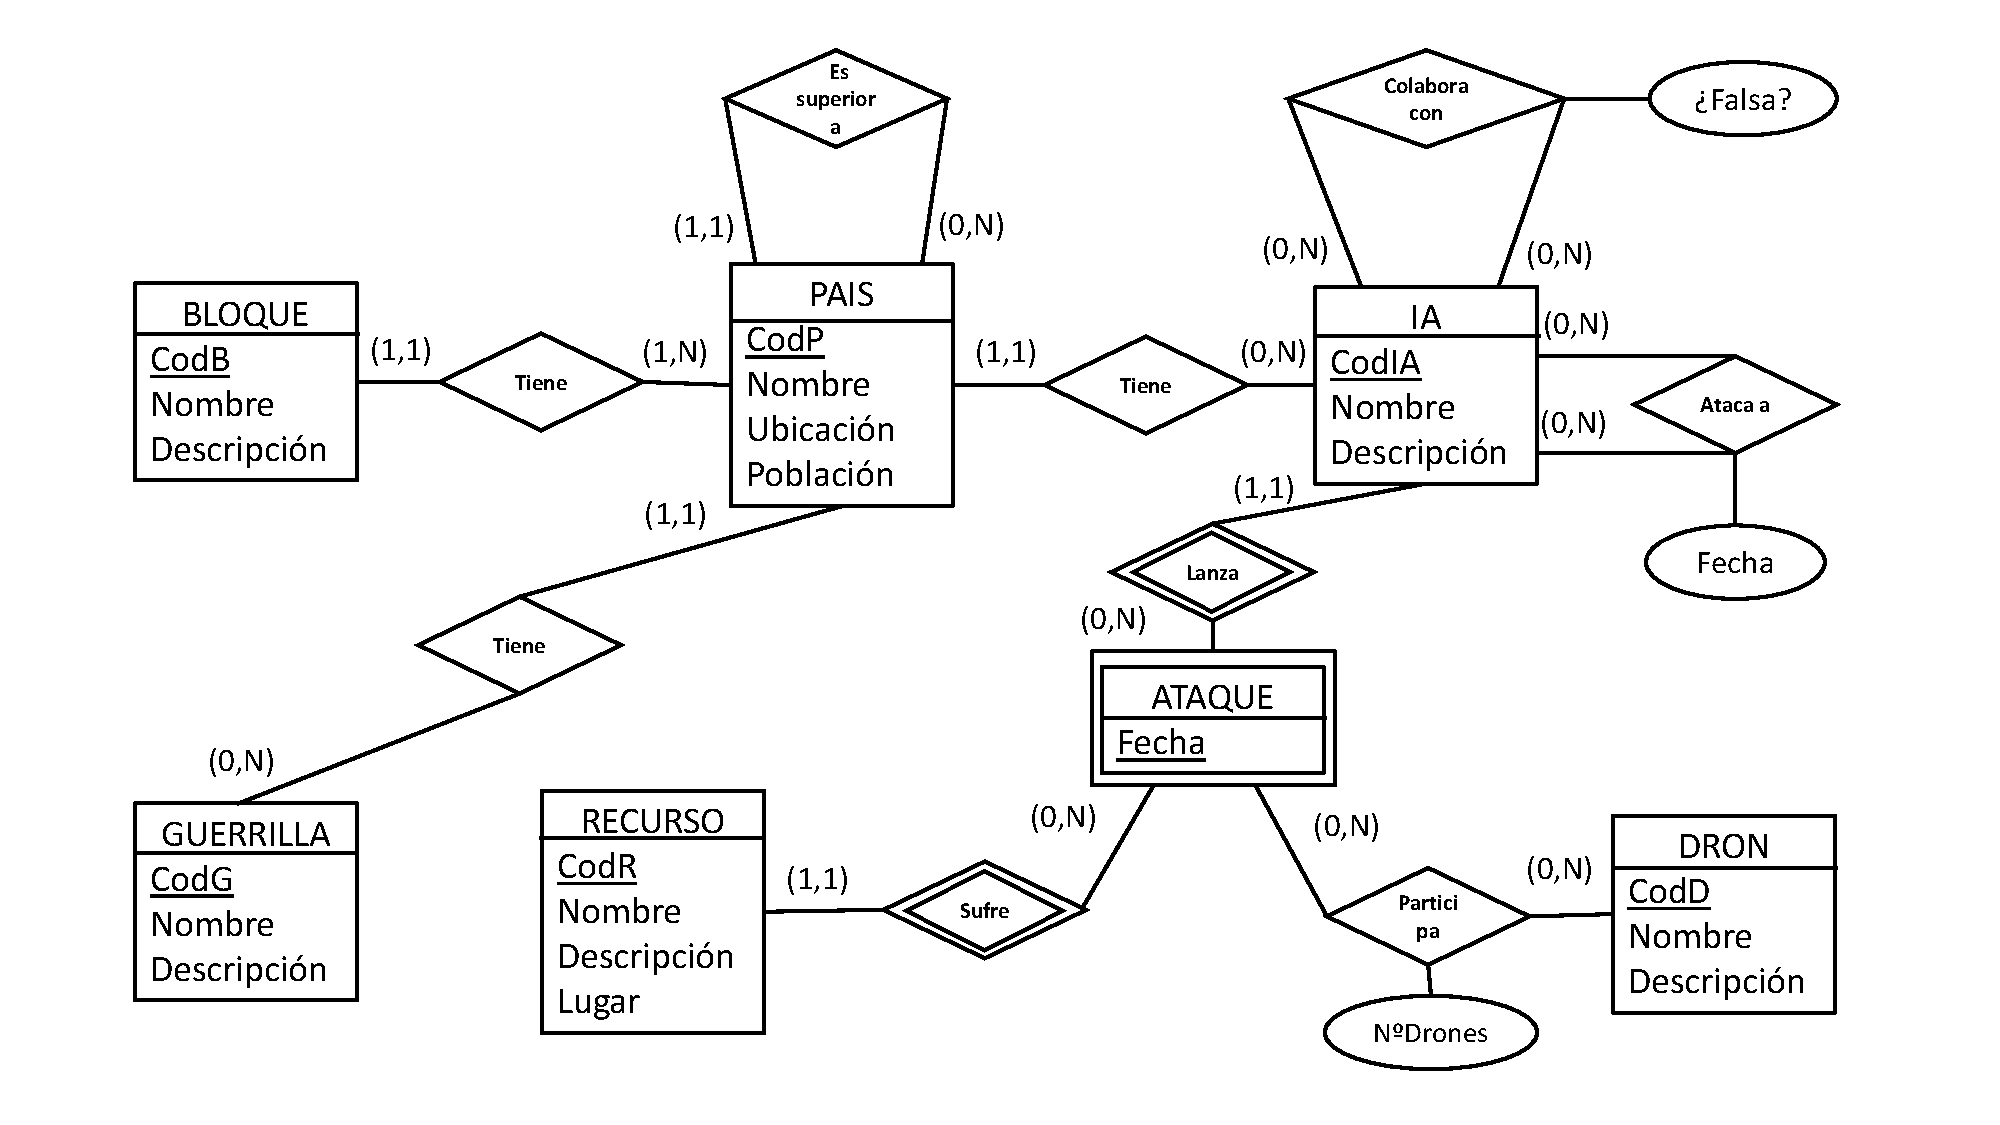
\includegraphics[width=\textwidth]{figs/bbdd-2022-2023-ordinaria/solucion-mer.pdf}
\end{solution}

\newpage
\question{\textbf{Consultas}}

Una cadena de muebles con nombre ``TLMT: Te lo montas tú'' necesita que hagamos algunas consultas sobre su base de datos. Para ello nos proporciona el diagrama relacional de una base de datos en producción. 
  
\begin{figure}[htpb!]
    \begin{center}
    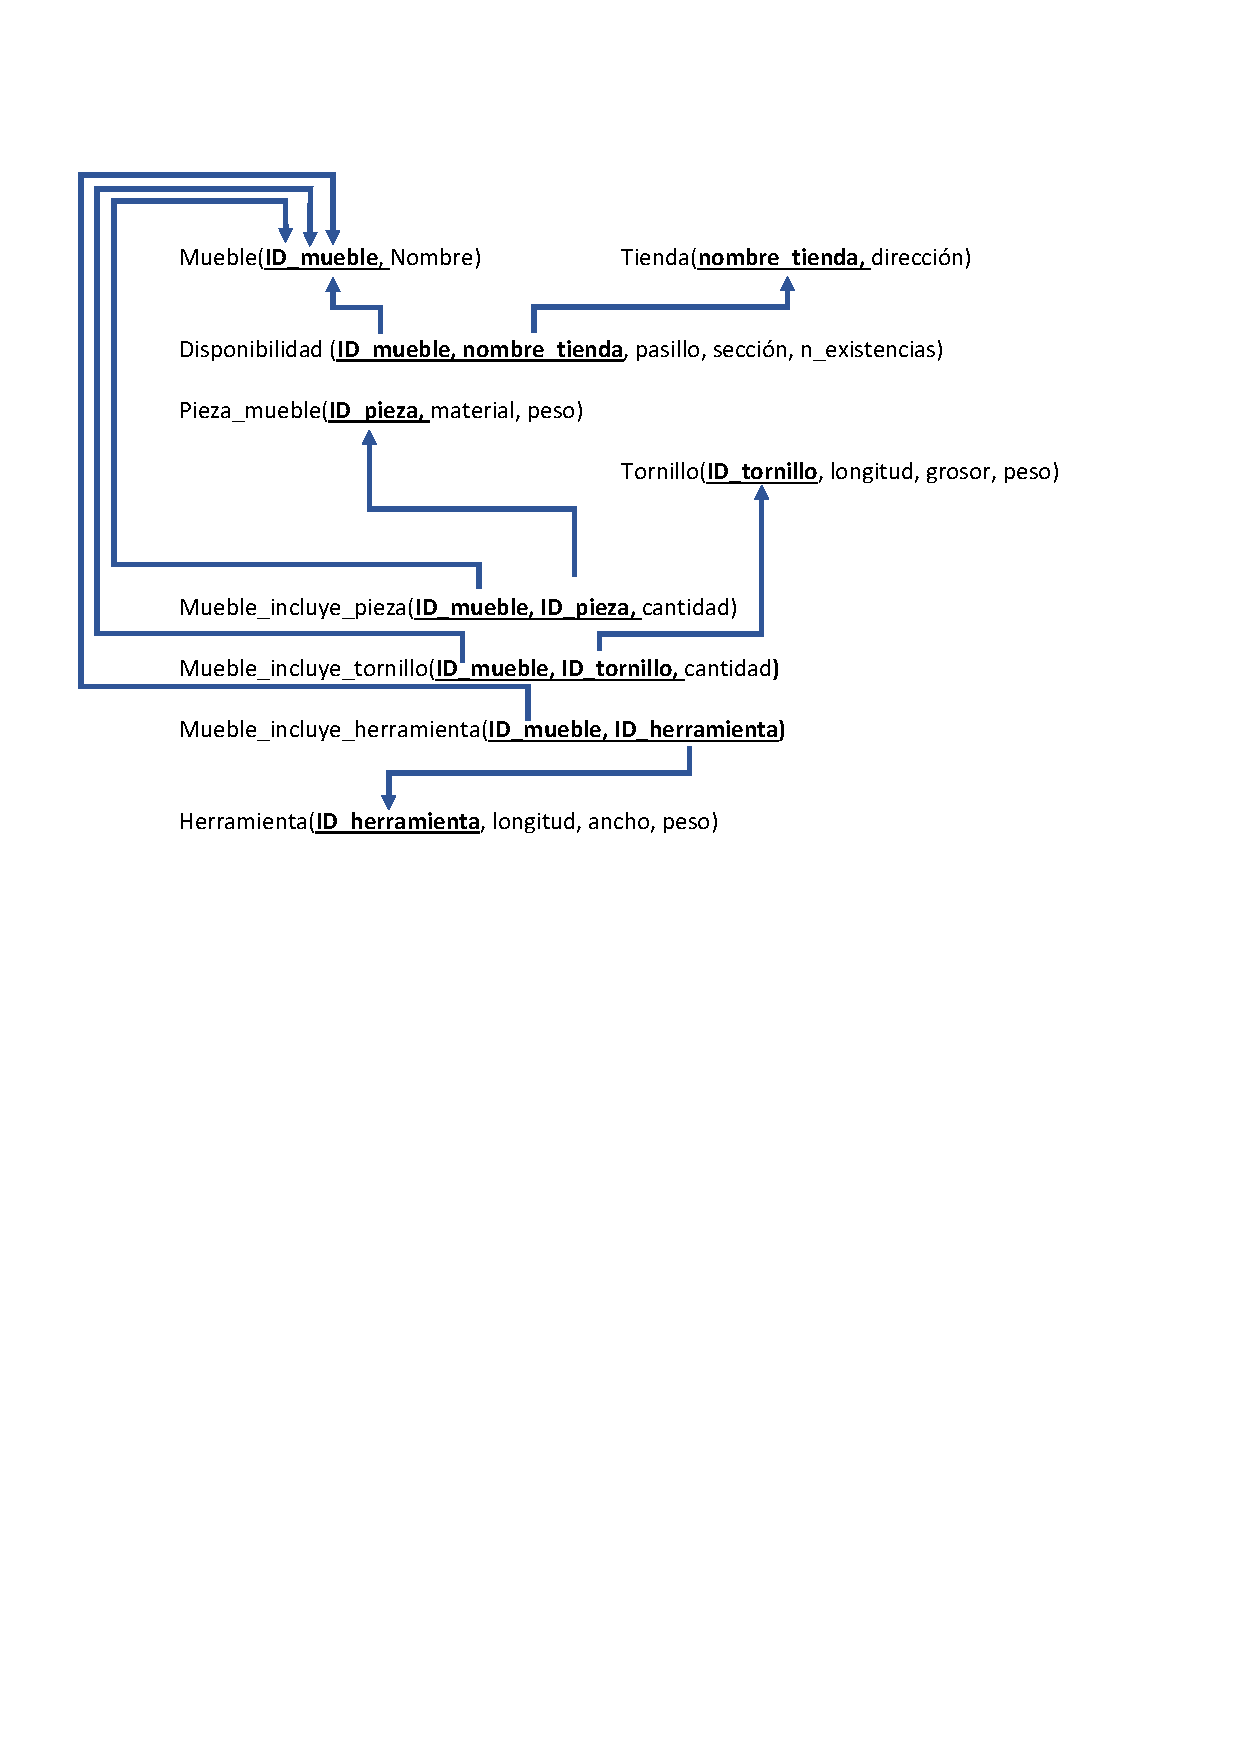
\includegraphics[width=1\textwidth]{figs/bbdd-2022-2023-ordinaria/tablasbloque2.pdf}
    \end{center}
\end{figure}
  
Se pide escribir la solución a las siguientes consultas.
\begin{parts}
\part\textbf{Álgebra relacional:}

\begin{subparts}
\subpart[\half] Obtener los pasillos y secciones en los que se encuentran la estantería ``Billy'' y la cajonera ``Alex'' en la tienda con nombre ``Ensanche de Vallecas''.
\begin{solution}
$\Pi_{pasillo,seccion}(\sigma_{nombre='Billy'}(Mueble)$

$\bowtie \sigma_{nombre\_tienda='Ensanche\ de\ Vallecas'}(Disponibilidad ))$

$\cup$

$\Pi_{pasillo,seccion}(\sigma_{nombre='Alex'}(Mueble)$

$\bowtie \sigma_{nombre\_tienda='Ensanche\ de\ Vallecas'}(Disponibilidad ))$
\end{solution}

\subpart[\half] Obtener el nombre de los muebles que se montan únicamente con tornillos de 3mm de longitud.
\begin{solution}
$\Pi_{nombre\_mueble}(Mueble \bowtie Mueble\_incluye\_tornillo$

$\bowtie \sigma_{longitud=3}(Tornillo))$

$-$

$\Pi_{nombre\_mueble}(Mueble \bowtie Mueble\_incluye\_tornillo$

$\bowtie \sigma_{longitud!=3}(Tornillo))$
\end{solution}

\subpart[\half] Obtener los muebles que incluyen todos los tornillos y herramientas.
\begin{solution}
$\Pi_{nombre\_mueble}(Mueble \bowtie \Pi_{id\_mueble, id\_tornillo}(Mueble\_incluye\_tornillo )$

$\div \Pi_{id\_tornillo}(Tornillo))$

$\cap$

$\Pi_{nombre\_mueble}(Mueble \bowtie \Pi_{id\_mueble, id\_herramienta}($

$Mueble\_incluye\_herramienta) \\ \div \Pi_{id\_herramienta}(Herramienta))$
\end{solution}


\end{subparts}

\part\textbf{SQL:} 

\begin{subparts}
\subpart[\half] Obtener el mueble que más tornillos requiere. Se debe obtener el id del mueble y el número de tornillos requeridos.
\begin{solution}
\begin{lstlisting}[language=sql]
SELECT mueble.id_mueble, SUM(mueble_incluye_tornillo.cantidad)
FROM mueble 
  INNER JOIN mueble_incluye_tornillo 
    ON mueble.id_mueble=mueble_incluye_tornillo.id_mueble
GROUP BY mueble_incluye_tornillo.id_mueble
HAVING SUM(mueble_incluye_tornillo.cantidad) 
  >= ALL (SELECT sum(cantidad)
          FROM mueble_incluye_tornillo
          GROUP BY id_mueble);
\end{lstlisting}
\end{solution}

\subpart[\half] Obtener aquellas tiendas que tienen al menos 10 unidades de todos los muebles (todos los que figuran en la tabla \textit{mueble}).

\begin{solution}[16em]
\begin{lstlisting}[language=sql]
SELECT * FROM tienda
WHERE NOT EXISTS (
  SELECT * FROM mueble
  WHERE NOT EXISTS(
    SELECT * 
    FROM disponibilidad
    WHERE tienda.nombre_tienda=disponibilidad.nombre_tienda
      AND mueble.id_mueble=disponibilidad.id_mueble
      AND disponibilidad.n_existencias >=10));
\end{lstlisting}
\end{solution}

\subpart[\half] Obtener el id de las piezas que comparten los muebles ``Helmer'' y ``Billy''.
\begin{solution}
\begin{lstlisting}[language=sql]
SELECT pieza.id_pieza
FROM pieza 
WHERE id_pieza IN (SELECT id_pieza
                   FROM mueble_incluye_pieza 
                     INNER JOIN mueble 
                       ON mueble_incluye_pieza.id_mueble=mueble.id_mueble
                   WHERE mueble.nombre='Helmer')
                     AND id_pieza IN (
                        SELECT id_pieza
                        FROM mueble_incluye_pieza 
                          INNER JOIN mueble 
                            ON mueble_incluye_pieza.id_mueble=mueble.id_mueble
                        WHERE mueble.nombre='Billy');
\end{lstlisting}
\end{solution}
\end{subparts}
\end{parts}

\newpage
\question{\textbf{Gestión}}

\begin{parts}

\part[1] En base al modelo relacional del Bloque 2, escriba una \emph{función} que devuelva el nombre de la tienda que disponga de la mayor cantidad de existencias de una pieza que se le pase como parámetro (ID\_pieza) a dicha función. Para ello se deberá utilizar un \texttt{CURSOR}.

\begin{solution}
\begin{lstlisting}[language=sql]
DELIMITER $$
CREATE FUNCTION maxTiendaStockPieza (id_pieza_param INTEGER)
RETURNS VARCHAR(250)
DETERMINISTIC
BEGIN
    DECLARE num_piezas, num_piezas_max INTEGER DEFAULT 0;
    DECLARE done INT DEFAULT FALSE;
    DECLARE nombre_tienda_aux, nombre_tienda_max VARCHAR(250);
    DECLARE cur1 CURSOR FOR SELECT nombre_tienda, 
                            SUM(n_existencias * cantidad)
                            FROM Disponibilidad INNER JOIN Mueble 
                            ON Disponibilidad.ID_mueble = Mueble.ID_mueble
                            INNER JOIN Mueble_incluye_pieza 
                            ON Mueble.ID_mueble = 
                            Mueble_incluye_pieza.ID_mueble
                            WHERE Mueble_incluye_pieza.id_pieza = id_pieza_param
                            GROUP BY nombre_tienda;
    DECLARE CONTINUE HANDLER FOR NOT FOUND SET done = TRUE;
    
    OPEN cur1;
    read_loop: LOOP
        FETCH cur1 INTO nombre_tienda_aux, num_piezas;
        IF done THEN
            LEAVE read_loop;
        END IF;
        IF num_piezas > num_piezas_max THEN 
            SET nombre_tienda_max = nombre_tienda_aux; 
            SET num_piezas_max = num_piezas; 
        END IF;
    END LOOP;
    CLOSE cur1;
    
    RETURN (nombre_tienda_max);
END$$
DELIMITER ;
\end{lstlisting}
\end{solution}

\newpage

\part[1] En base al modelo relacional del Bloque 2, en primer lugar, generar la \emph{sentencia SQL de creación de una nueva tabla} `traspaso\_existencias\_tiendas' con la siguiente estructura:
\begin{table}[h]
    \centering
    \begin{tabular}{|c|c|c|c|c|}
    \hline
            nombre\_tienda\_origen & nombre\_tienda\_destino & id\_mueble & cantidad & fecha \\
            \hline
            ... & ... & ... & ... & ...\\
        \hline
    \end{tabular}
    %\caption{Caption}
    \label{tab:pedidosalm}
\end{table}
\\ Dicha tabla deberá contener las claves foráneas correspondientes. Seguidamente crear un \emph{trigger} que compruebe que cuando una tienda se quede con un número de existencias menor a 5 de un mueble a causa de una actualización de su \textit{stock}, inserte en la nueva tabla creada un registro para pedir un traspaso de existencias. Dicho traspaso deberá ser de 3 muebles, y se deberá realizar a dicha tienda procedente de una de las tiendas que tenga el mayor numero de existencias de ese mueble en ese momento. 
    
\begin{solution}
\begin{lstlisting}[language=sql]
CREATE TABLE traspaso_existencias_tiendas(
nombre_tienda_origen VARCHAR(250) NOT NULL,
nombre_tienda_destino VARCHAR(250) NOT NULL,
id_mueble INTEGER NOT NULL,
cantidad INTEGER NOT NULL,
fecha DATE NOT NULL,
PRIMARY KEY(nombre_tienda_origen,nombre_tienda_destino,id_mueble,fecha),
FOREIGN KEY(nombre_tienda_origen) REFERENCES Tienda(nombre_tienda),
FOREIGN KEY(nombre_tienda_destino) REFERENCES Tienda(nombre_tienda),
FOREIGN KEY(id_mueble) REFERENCES Mueble(id_mueble),
)

DELIMITER $$
CREATE TRIGGER chequeoDeExistencias
AFTER UPDATE ON Disponibilidad
FOR EACH ROW
BEGIN
    DECLARE tienda INTEGER;

    IF NEW.n_existencias < 5 THEN
    
        SELECT nombre_tienda INTO tienda
        FROM Disponibilidad
        WHERE id_mueble = NEW.id_mueble
        AND n_existencias = (SELECT MAX(n_existencias) FROM Disponibilidad
        WHERE id_mueble = NEW.id_mueble)
        LIMIT 1;

        INSERT INTO traspaso_existencias_tiendas 
        (nombre_tienda_origen, nombre_tienda_destino, id_mueble, cantidad, 
        fecha) 
        VALUES (tienda, NEW.nombre_tienda, NEW.ID_mueble, 3, CURDATE()); 
    END IF;
END$$
DELIMITER ;
\end{lstlisting}
\end{solution}
    
\end{parts}

\newpage
\question{\textbf{Ficheros}}

Tomando como referencia el siguiente archivo XML, resuelva las preguntas a continuación.   

\begin{verbatim}
<?xml version=“1.0”>
<libros>
    <libro>
        <isbn> 9781600108952 </isbn>
        <titulo> Dungeons & Dragons </titulo>
        <autores>
            <autor>
                <nombre> Ernest</nombre>
                <apellido> Gary Gygax</apellido>
                <email> gygax@gmail.com </email>
            </autor>
            <autor>
                <nombre> David </nombre>
                <apellido> Lance Arneson </apellido>
                <email> dave@gmail.com </email>
            </autor>
        </autores>
        <precio> 78.45 </precio>
        <año> 1974 </año>
    </libro>
    ...
</libros>
\end{verbatim}

\begin{parts}

\part [\half] Obtener el nombre y apellidos mediante una consulta \textbf{XQUERY}, de aquellos autores que han escrito libros que valen más de 80\euro. Es necesario mostrar los resultados con el siguiente formato:
\texttt{<autor> nombre - apellido </autor> ... <autor> nombre - apellido </autor>}
\begin{solution}
\begin{verbatim}
for $x in //libro
where $x/precio > 80
return  for $y in $x/autores 
		return <autor>{$y/autor/nombre/text()} - 
            {$y/autor/apellido/text()}</autor>
\end{verbatim}
\end{solution}

\part [\half] Realice una consulta \textbf{XPATH} que devuelva el título de aquellos libros que cuesten más de 70\euro{}.
\begin{solution}
\begin{verbatim}
/libros/libro[precio>70]/titulo
\end{verbatim}
\end{solution}
  
\end{parts}

\newpage
\question{\textbf{Programación contra bases de datos}}

\begin{parts}
\part[1] El siguiente modelo relacional pertenece a una base de datos de una gestora de comercios farmacéuticos.

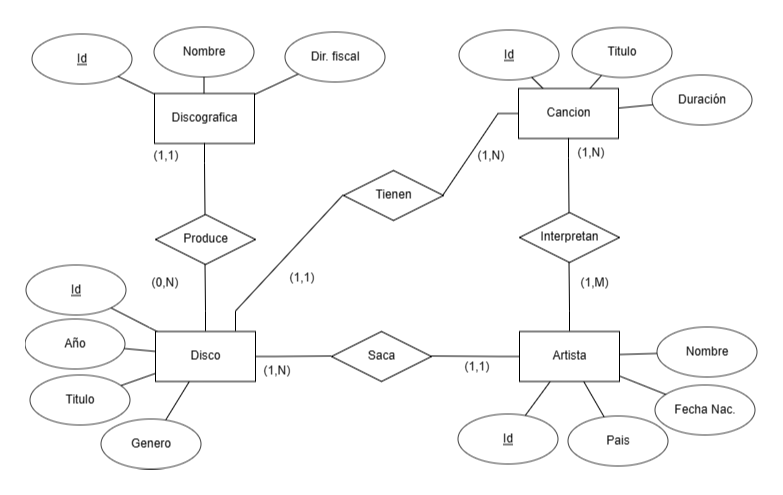
\includegraphics[width=0.9\textwidth]{figs/bbdd-2022-2023-ordinaria/mer-hibernate.png}

En dicha base de datos se quiere almacenar las distintas discográficas que producen discos. Un disco pertenece a un artista y a una discográfica. El disco, como es lógico, se compone de distintas canciones. Esas canciones a su vez pueden estar interpretadas por uno o varios artistas. Realice el etiquetado de clases y sus atributos para que mediante el ORM \textbf{Hibernate} de Java pueda realizar la conexión con la base de datos satisfactoriamente cumpliendo con el modelo relacional mostrado anteriormente.
\vspace{5mm}
    
\begin{verbatim}
public class Discografica {

private Long id;

private String nombre;

private String domicilio_fiscal;

private Set<Disco> discos;
    
/*Constructor de la clase, getters, setters,...*/
}

            
public class Artista {

private Long id;

private String nombre;

private String pais;

private Date fecha;

private Set<Disco> discos;

private Set<Cancion> canciones;
    
/*Constructor de la clase, getters, setters,...*/
}


public class Disco {

private Long did;

private String titulo;

private Integer año;

private String genero;

private Discografica discografica;

private Artista artista;

private Set<Cancion> canciones;

/*Constructor de la clase, getters, setters,...*/
}


public class Cancion {

private Long id;

private String titulo;

private Time duracion;

private Set<Artista> artistas;

private Disco disco;
    
/*Constructor de la clase, getters, setters,...*/
}
\end{verbatim}

\begin{solution}
\begin{verbatim}
@Entity
@Table(name="Discography")
public class Discografica {
@Id
@GeneratedValue
@Column(name="id", unique = true, nullable = false)
private Long id;
@Column(name="name", nullable = false)
private String nombre;
@Column(name="fiscalAdd", nullable = false)
private String domicilio_fiscal;
@OneToMany(mappedBy = "discografia")
private Set<Disco> discos;
/*Constructor de la clase, getters, setters,...*/
}

@Entity
@Table(name="Artist")
public class Artista {
@Id
@GeneratedValue
@Column(name="id", unique = true, nullable = false)
private Long id;
@Column(name="name")
private String nombre;
@Column(name = "country")
private String pais;
@Column(name = "birthdate")
private Date fecha;
@OneToMany(mappedBy = "artista")
private Set<Disco> discos;
@ManyToMany(mappedBy="artistas")
private Set<Cancion> canciones;
/*Constructor de la clase, getters, setters,...*/
}

@Entity
@Table(name="Disc")
public class Disco{
@Id
@GeneratedValue
@Column(name="id", unique = true, nullable = false)
private Long did;
@Column(name="tittle", nullable = false)
private String titulo;
@Column(name="year", nullable = false)
private Integer año;
@Column(name="genre", nullable = false)
private String genero;
@ManyToOne(optional = false)
@JoinColumn(name = "discos")
private Discografica discografica;
@ManyToOne(optional = false)
@JoinColumn(name = "artista")
private Artista artista;
@OneToMany(mappedBy = "disco")
private Set<Cancion> canciones;
/*Constructor de la clase, getters, setters,...*/
}

@Entity
@Table(name = "Song")
public class Cancion {
@Id
@GeneratedValue
@Column(name="id", unique = true, nullable = false)
private Long id;
@Column(name="tittle", nullable = false)
private String titulo;
@Column(name="duration", nullable = false)
private Time duracion;
@ManyToMany()
@JoinTable(name = "Play")
private Set<Artista> artistas;
@ManyToOne(optional = false)
@JoinColumn(name = "did")
private Disco disco;
/*Constructor de la clase, getters, setters,...*/
}
\end{verbatim}
\end{solution}
\end{parts}

\end{questions}

\end{document}